\chapter{Urban Data}
This chapter aims to describe the nature of urban data --- the sources, classification, and available formats. To some extent the term \textit{urban data} is somewhat simmilar to other buzzwords, such as \textit{big data}. As there is no official definition of the term \textit{urban data}, it is often explaied by giving a list of examples, such as transport data or socio-economic maps. The urban data is a subject of study in several fields, one of which is the Urban Informatics.

\section{Urban Informatics}
In 2011, Forth et al. \cite{foth2011urban} described Urban Informatics as a separate field of study. It focuses on three key aspects --- place, technology, and people in the context of urban environments. The urban environment is described as a \textit{"complex techno-social network; the city only meaningfully exists when a sustained stream of people occupies it"} \cite{foth2011urban}. The authors outline and study four dominant trends: the emergence of ubiquitous computing, the accessibility of real-time information, informed sustainability, and planning based on citizen participation. 

One of the goals of Urban Informatics is to help developing communication channels between local authorities and citizens. Moreover, thanks to the gathered information, the citizens can, directly and indirectly, influence the development of the urban area. The communication channels, as understood by Urban Informatics, are omnidirectional. 

\section{Sources of Urban Data}
This section contains description of three main urban data sources. This clasification is based on the summary presented in \cite{robinson2012street}. The urban data sources include mainly governments and local administrative institutions. Additionaly, the data is gathered and received through devices that are part of the ubicomp device system. The third source of urban data consists of online services, such as social networks. 

\paragraph{Open Data}
The most prominent source of data are governments and local institutions. The data is commonly released in several open formats, which are further described in the section \ref{sec:formats}. This data often includes maps, building layouts, terrain models, technical metadata, public transport data, etc. The formats range from generic CSV or SQLite-based to domain-specific DWG, CityGML, etc.   
The data presented earlier are mainly static; some cities also offer real-time information about weather or public transport vehicle locations. 

\paragraph{Ubicomp} Mark Weiser first introduced Ubiquitous Computing in 1991 \cite{weiser1991computer}. The concept of ubicomp relies on small embedded computers, which communicate together and allow for seamless interaction between users and technology. Accoring to \cite{zheng2011urban}, the ubiquitous information's impact on the city level became the focus of study in a separate field called Urban Computing. In the spirit of ubiquitous computing, there is an emerging field of Participatory Sensing \cite{burke2006participatory}, which enables gathering data from devices of individual users. The design of the participation model focuses on data credibility, security, and privacy protection. One of the applications of Participatory Sensing is the use of the gathered data for urban planning. 

\paragraph{Online services}
Personal data can also be acquired from social networks or mobile phone carriers. Online platforms usually support geotagging, adding geospatial metadata to the content posted online. The content can be easily queried based on the selected location. Alternatively, the citizens' location can be tracked via their mobile phone directly by carriers using the individual base transceiver stations (BTS).  From the perspective of Urban Informatics, the aforementioned data sources enable creating richer urban area models. 

\section{Urban Data Domains}
There is no official classification of the urban data. However, open data portals usually use custom classification schemes, which are either domain or format-based. Based on the available open data catalogues of the cities in 5 Cities Connect\footnote{Prague has been recently invited into the 5CC initiative} group \cite{5CC}, a list of domain classes has been assembled, see table \ref{tab:opendata}. The listed domains are either of significant importance or have appeared across a majority of the reviewed catalogues.  


% Please add the following required packages to your document preamble:
% \usepackage{booktabs}
\begin{table}[]
    \resizebox{0.9\textwidth}{!}{
    \begin{tabular}{@{}lllllll@{}}
    \toprule
    Domain                   & Hamburg & Vienna & Rotterdam & Helsinki & Singapur & Prague \\ \midrule
    Buildings                & x       & x      & x         & x        &          & x      \\
    Population and Work      & x       & x      &           & x        & x        & x      \\
    Technical infrastructure & x       & x      &           & x        & x        & x      \\
    Transport                & x       & x      & x         & x        & x        & x      \\
    Geology                  & x       &        & x         &          &          & x      \\
    Noise maps               &         & x      &           & x        &          & x      \\
    Environment and Nature   & x       & x      & x         & x        & x        & x      \\
    Ortographic maps         & x       & x      & x         & x        & x        & x      \\
    Public services          & x       & x      & x         & x        & x        & x      \\
    Terrain                  &         & x      & x         & x        &          & x      \\
    Air Quality              &         &        & x         & x        & x        & x      \\
    Zoning Plan              &         & x      & x         & x        & x        & x      \\ \bottomrule
    \end{tabular}}
    \caption{Urban data classes availability on open data portals}
    \label{tab:opendata}
\end{table}


\section{File Formats}
\label{sec:formats}
This section describes the file formas used to store various urban data. Some of these file formats are proprietary; however, from the perspective of application development, open formats are more attractive. 

\paragraph{Esri Shapefiles} 
Esri Shapefile \cite{esri1998shapefile} is generally a vector data file format for a geographic information system. A single shapefile consists of several files; the minimal set of files necessary for correct data interpretation is  DBF, SHP, and PRJ file: 

\begin{description}[noitemsep]
    \item[SHP] contains the actual geometry,
    \item[DBF] contains the attributes and indexes,
    \item[PRJ] describes the coordinate reference system.  
\end{description}
In the original specification \cite{esri1998shapefile}, SHX is also a mandatory file. Still, the file only allows to accelerate the queries and is not required for the data to be displayed correctly. The Shapefile format is well documented, and there is a range of existing importers in various languages. 


\paragraph{CityGML and CityJSON}
CityGML \cite{groger2012ogc} is an XML-based file format designed to capture the structure and metadata of 3D city models. The aim of the development is to come up with a standardized and sustainable way of storing urban data. There is a JSON-based version of CityGML - CityJSON \cite{ledoux2019cityjson}. Despite minor differences, these two standards are mostly compatible. From the practical point of view, the CityJSON format is much less verbose and thus easily parsable. Both CityGML and CityJSON are open formats; there are convertors and importers available .

\paragraph{GeoJSON}
Another JSON-based standard is the GeoJSON format. This GeoJSON structure is quite simple; the file can describe a set of primitive geometry objects such as lines, lines, or polygons. Each primitive can have a variable number of properties, which can be completely arbitrary. The GeoJSON file usually describes data such as networks or areas. Compared to CityJSON, GeoJSON is not suitable for representing hierarchies, which usually naturally appear in building geometry and its components. GeoJSON is an open format, it is fairly simple to write an importer for this format, and there are several available, see \cite{cityJSONconvert, cityGMLimport}. 

\paragraph{DGN and DWG}
Both of these formats are proprietary vector formats used by CAD editors, such as AutoCAD. A reader for the DWG format is a part of RealDWG developer suite created by Autodesk \cite{autodeskRealDWG}. Its license is incompatible with most free software licenses. As a result, no open tools contain an effective importer for the DWG file format. There is no official free DWG SDK; the software for importing and converting DWG is a part of software offered by OpenDesignAlliance (ODA) \cite{alliance1998open}. Some sort of DWG and DGN loading capabilities are implemented in the GDAL framework \cite{GDALframework}.

\paragraph{BIM and IFC}
Based on \cite{TANG2017311}, Building Information Model (BIM) is the common name for all data relevant to an architectural structure --- the plans, costs, changes over time, etc. Industry Foundation Classes (IFC) is a data model designed for architectural, building, and construction data. It is a platform-neutral and open file format. In some states, the IFC has been legally established as the standard exchange format for public project data. Like Shapefiles, IFC is not a single file; there are many available IFC versions, and the development of newer ones is underway. On the other hand, contrary to Shapefiles, each IFC file version should include the same data; the only difference is in the encoding. 


\section{Models Based on Urban Data}
\label{sec:analytics}
Urban data alone is not always a sufficient input for city planning. The main issue is the static nature of the data. According to Ira Winder \cite{winderLUPA}, analytical models presented as interactive simulations are often more suitable for the purpouses of planning. The models help answer questions. There is no guarantee the models are correct; complex models can be just as useful as the simple ones. 

\begin{figure}[h]
    \centering
    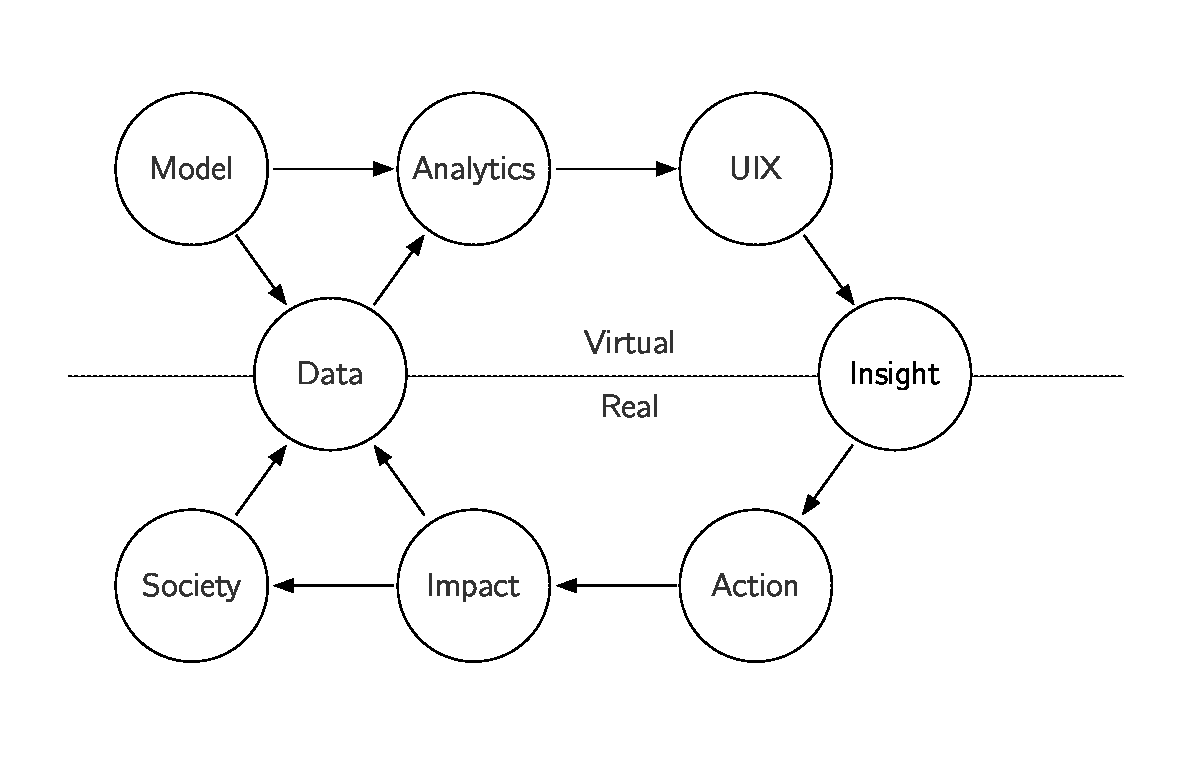
\includegraphics[width=0.8\linewidth]{figures/Loop2.pdf}
    \caption{Sociotechnical system model \cite{winderLoop}}
    \label{fig:loop2}
\end{figure}

In a talk given by Ira \cite{winderLoop}, he describes the paradigm of generating insight from data, which is illustrated in figure \ref{fig:loop2}. He emphesises the role of the user interface, which is essential in getting familiar with the actual data and analytics. The generated insight influences further planning and development. The impact of these actions has the potential to generate new data which feeds back into the loop. The step from data to analytics can be rather intensive and involves creating analytical models. 

